\chapter{Intrusion Detection}
\begin{figure}[htbp]
   \centering
   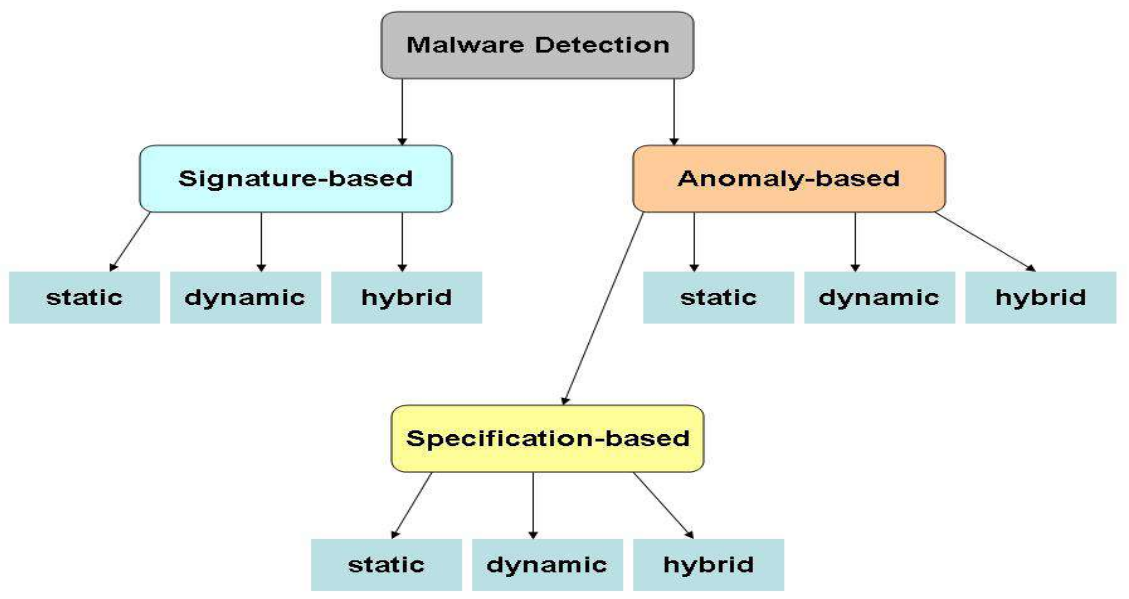
\includegraphics{images/IntrusionDetection_schema.png}
   \caption{Intrusion Detection Taxonomy}
   \label{fig:IntrusionDetection_taxonomy}
\end{figure}

\labelitemize{
   \textbf{INPUT-EVENTS}
}{
   \begin{enumerate}
      \item End-point events
         \begin{enumerate}
            \item  Invocation to OS
            \item  Memory analysis
            \item  Files that are downloaded
            \item  Programs that are executed
         \end{enumerate}
      \item Network events
         \begin{enumerate}
            \item Contents of packets that are transmitted
            \item Information transmitted on a circuit
         \end{enumerate}
      \end{enumerate}
      }
      
\textbf{Networks events} are generated by a module that monitors ongoing communication, i.e. a \textbf{packer sniffer}.\\
This poses two problems:
\begin{enumerate}
   \item \textit{Lost messages}, since the sniffer cannot slow down the communication it is sniffing
   \item \textit{Assumptions} on the \textit{behavior} of the receiving node
\end{enumerate}
There are \textit{\textbf{evasion} attacks} where the attacker transmits \textbf{fake packets} to increase the computational load od the detection,
exploiting fake checksum, overlapping fragments etc.

\section{Anomaly Based}
The behavior of the target system is observed for a time interval and a \textbf{learning model} is built representing the \textit{normal} behavior.\\
Note that \textbf{learning} implies discovering parameters such as:
\begin{itemize}
   \item \textbf{Services} that are used and time of the usage
   \item When users \textbf{log in} and the length of their \textbf{sessions}
   \item User \textbf{requests} and \textbf{OS functions} they invoke
   \item Computation and communication \textbf{bandwidths} used
\end{itemize}
After the learning phase, any behavior that is too \textit{far} from the model that has
been built is defined as an \textbf{anomaly} due to an \textit{ongoing intrusion}.\nl
Clearly the critical parameters are the amount of \textbf{information} acquired during the learning phase and the \textbf{threshold} on the \textit{"distance"}.
Sometimes continuous learning is preferred since the normal behavior \textbf{changes} as time passes.

\begin{enumerate}
   \item \textbf{Dynamic}:
   Information on a program behavior are collected by executing the program
   \item \textbf{Static}:
   A static analysis returns information on the program behavior\\
   e.g. the OS functions it calls, information on the call order, etc.
   \item \textbf{Hybrid}:
   Dynamic collection of information to cover lack of information in the output of the static analysis
\end{enumerate}

\subsection{Specification Based}
The key point here is that the so-called normal network behaviour is not deduced by observing programs behaviour over time,
instead by what are the running programs and what they should do according to their specification. 